%\cleardoublepage

\chapter{DESIGN TOOLS}
\label{ch:SWHEModel}

In this chapter, tools are developed to aid in SWHP system design. In the following sections, handbook style design diagrams for space heating and space cooling are developed which are based on the experimentally derived heat transfer correlations described in Chapter \ref{ch:Correlation}.

\section{Design Graph Derivation}
\label{sec:DesignTools:Derivation}

To develop the diagrams, a simulation was developed using the previously developed outside convection correlations. In the simulation the zone load was fixed at 1 ton (3,517 W) for the case of space cooling and at 12 MBTUh (3,517 W) for the case of space heating. Other parameters such as tube size, coil geometry, circulating fluid, fluid flow rate, lake temperature, heat pump COP, tube material, tube schedule, tube fouling resistance, and surface water characteristics were also held constant for each individual case. Then, to generate the diagrams, a range of coil entering fluid temperatures were input into the model. From this, the model determined the coil length required to meet the zone load. This method allowed the zone heat transfer rate per required length of coil to be determined, which could then be plotted against approach temperature. Approach temperature is defined as the temperature difference between the coil exiting fluid temperature and the lake temperature.

\section{Space Cooling Design Graphs}
\label{sec:DesignTools:SpcCooling}

In this section design diagrams for space cooling are given.  The design diagrams give the required installed pipe length for the given design conditions plotted against the approach temperature difference. For all design diagrams, the various design options are compared against the ``typical" case. This case is defined as a mid-way point between what is being called the ``best-case" and ``worst-case" designs. Here, ``best" case is used to describe the set of SWHP system and SWHE parameters that are most favorable to SWHE performance within the context of these design diagrams. The ``worst" case is used to describe the SWHP and SWHE system parameters that are least favorable to system performance. 

Figure \ref{fig:DesignTools:SpcCooling:BestWorst} shows the required pipe length plotted against approach temperature for the ``typical," ``best," and ``worst" HDPE design cases. Table \ref{tab:DesignTools:SpcCooling:BestWorstParam} shows the SWHP systems and SWHE parameters that are fixed for each respective case. Heat pump COP is constant and based on the average COP from four separate off-the-shelf water-air heat pumps with a capacity from 1-3 tons at the expected heat pump entering fluid temperatures. ``Best" and ``worst" case surface water temperatures were taken from the high and low values from the isotherm plots obtained from \cite{Selvakumar2013}, respectively. Later, we will explain why the 95$^\circ$F (35$^\circ$C) lake temperature was selected as the ``best" case and why the 50$^\circ$F (10$^\circ$C) lake was selected as the ``worst" case. The rest of the parameters outlined in Table \ref{tab:DesignTools:SpcCooling:BestWorstParam} will be given more discussion later in the section.

	\begin{figure}
		\centering
		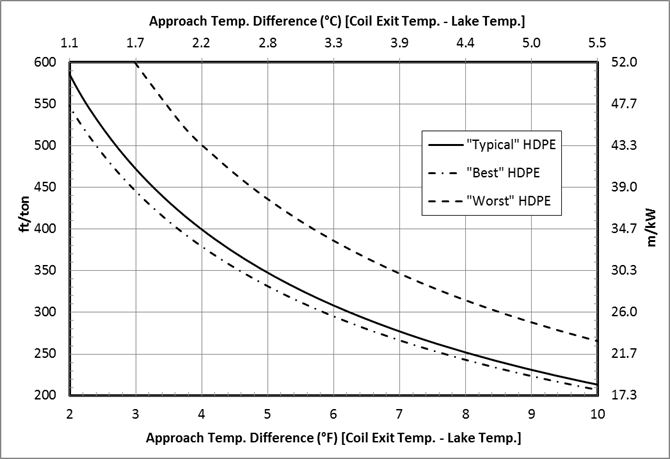
\includegraphics[width=0.8\textwidth]{BestWorst.png}
		\caption{``Best" and ``worst" case HDPE design diagram}
		\label{fig:DesignTools:SpcCooling:BestWorst}
	\end{figure}

	\begin{table}[h]
		\centering
		\caption{Parameters for the ``best" and ``worst" cases}
		\label{tab:DesignTools:SpcCooling:BestWorstParam}
		\begin{tabular}{r c c c}
		\hline
		& ``Typical" HDPE & ``Best" HDPE & ``Worst" HDPE \\
		\hline\hline
		HP $\mbox{COP}_h$ & 4 & 2.9 & 5.5 \\
		\hline
		Lake Temp & 70$^\circ$F (21.1$^\circ$C) & 95$^\circ$F (35$^\circ$C) & 50$^\circ$F (10$^\circ$C) \\
		\hline
		Vert.\ Spacing & 2.625 in.\ (67 mm) & 4.125 in.\ (105 mm) & 1.3 in.\ (33 mm)\\
		\hline
		Horiz.\ Spacing & 2.625 in.\ (67 mm) & 4.125 in.\ (105 mm) & 1.3 in.\ (33 mm) \\
		\hline
		Tube Size & 1 in.\ (25 mm) & 1-1/4 in.\ (32 mm) & 3/4 in.\ (19 mm) \\
		\hline
		Tube Schedule & \multicolumn{3}{c}{SDR-11} \\
		\hline
		Tube Material & \multicolumn{3}{c}{HDPE PE 3408} \\
		\hline
		Flow Rate & \multicolumn{3}{c}{3 gpm (11.4 L/min)} \\
		\hline
		Space Cooling & \multicolumn{3}{c}{1 ton (3,517 W)} \\
		\hline
		Circ. Fluid & 12.5\% PG & Water & 25\% PG \\
		\hline
		\multirow{2}{*}{Ext.\ Fouling} & \multirow{2}{*}{None} & \multirow{2}{*}{None} & 0.00053 hr-ft$^2$-$^\circ$F/BTU \\
		 & & & 0.003 m$^2$-$^\circ$C/W \\
		\hline
		\multirow{2}{*}{Int.\ Fouling} & \multirow{2}{*}{None} & \multirow{2}{*}{None} & 0.000175 hr-ft$^2$-$^\circ$F/BTU \\
		 & & & 0.001 m$^2$-$^\circ$C/W \\
		 \hline
		Surface Water & \multirow{2}{*}{Pond} & \multirow{2}{*}{Pond} & \multirow{2}{*}{Pond} \\
		Charachteristics & & & \\
		\hline
		\end{tabular}
	\end{table}
	
Figure \ref{fig:DesignTools:SpcCooling:BestWorstPE} shows the percent error between the ``typical" HDPE case and the ``best" and ``worst" cases. The ``typical" HDPE case is taken as the base case. From this figure, we can see that the percent difference between the ``typical" and ``best" case ranges from 4-8\%. This means that at 4-8\% reduction in installed SWHE length per ton (3,517 W) of space cooling could be achieved if the ``best" method were applied. A 24\% increase in installed SWHE length is required if the ``worst" practice is applied.
	
	\begin{figure}
		\centering
		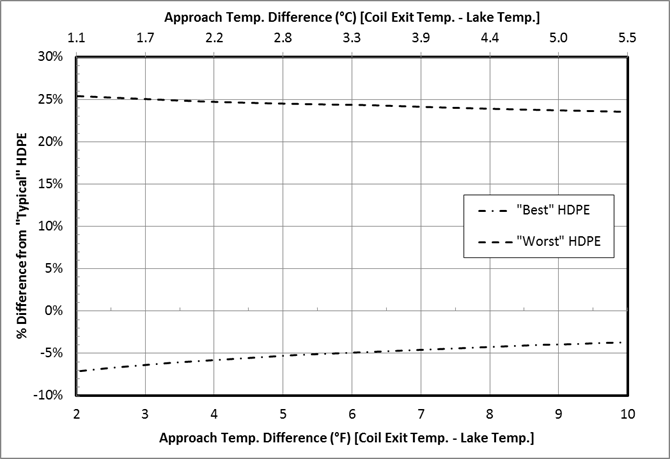
\includegraphics[width=0.8\textwidth]{BestWorstPE.png}
		\caption{``Best" and ``worst" case HDPE design diagram percent error}
		\label{fig:DesignTools:SpcCooling:BestWorstPE}
	\end{figure}
	
Figure \ref{fig:DesignTools:SpcCooling:BestWorstCopper} shows the ``typical," ``best," and ``worst" cases for copper SWHEs. All parameters shown in Table \ref{tab:DesignTools:SpcCooling:BestWorstParam}, with the exception of the tube material, are identical for this copper SWHE design diagram. Figure \ref{fig:DesignTools:SpcCooling:BestWorstCopperPE} shows the percent difference from the ``typcial" copper case similar to what was described previously for the HDPE SWHEs.
	
	\begin{figure}
		\centering
		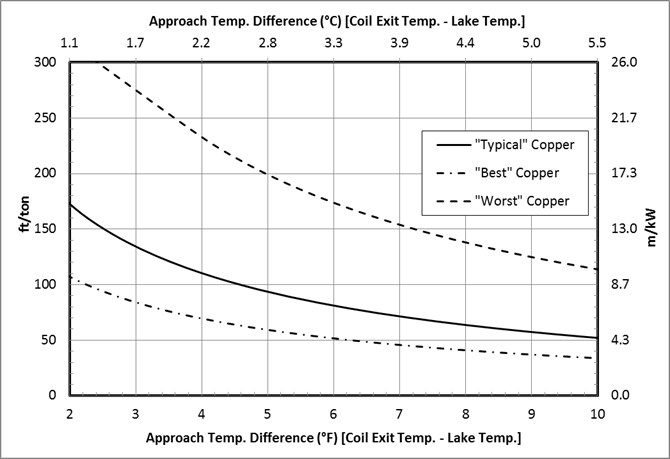
\includegraphics[width=0.8\textwidth]{BestWorstCopper.png}
		\caption{``Best-case" and ``worst-case" copper SWHE design diagram}
		\label{fig:DesignTools:SpcCooling:BestWorstCopper}
	\end{figure}
	
For Figure \ref{fig:DesignTools:SpcCooling:BestWorstCopperPE} we see that changing to the ``best" case parameters for the copper SHWE could result in a 40\% reduction in required SWHE tube length. However, for the ``worst" case, an increase of 105-118\% would be required. The copper SHWE is much more sensitive to the various cases because the pipe conduction resistance is no longer the dominate thermal resistance. For HDPE SWHEs, the pipe thermal resistance often makes up nearly half of the total thermal resistance, whereas for copper SWHEs, the pipe conduction resistance is negligible.
	
	\begin{figure}
		\centering
		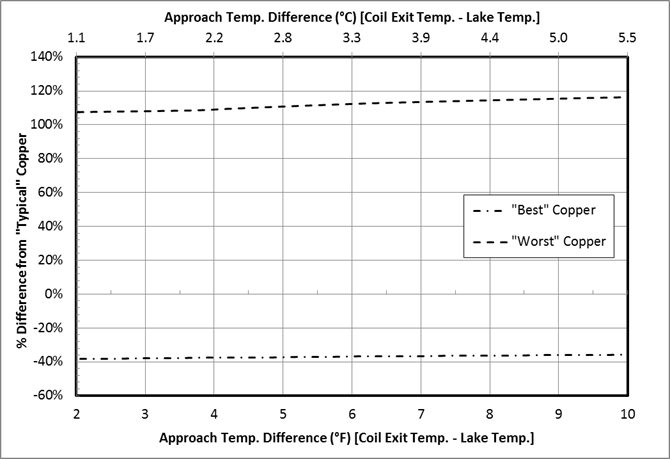
\includegraphics[width=0.8\textwidth]{BestWorstCopperPE.png}
		\caption{``Best-case" and ``worst-case" copper SWHE design diagram percent error}
		\label{fig:DesignTools:SpcCooling:BestWorstCopperPE}
	\end{figure}

From Figures \ref{fig:DesignTools:SpcCooling:BestWorst} and \ref{fig:DesignTools:SpcCooling:BestWorstCopper} we have established our ``typical" HDPE and copper cases. These will be the base cases for comparison purposes throughout the remainder of this section.


In Figure \ref{fig:DesignTools:SpcCooling:HPCOP}, variations in required pipe length due to variations in heat pump COP can be seen. From the figure, we see that for space cooling applications, lower heat pump COPs will require longer installed pipe lengths for a fixed zone load. The reverse is also true in that higher COPs will require less installed pipe. A drop in heat pump COP signifies a decrease in heat pump efficiency, i.e. more work is required for a constant output and more compressor heat must be rejected. This decrease in efficiency is reflected in the design diagrams by an increase in required pipe length.

	\begin{figure}
		\centering
		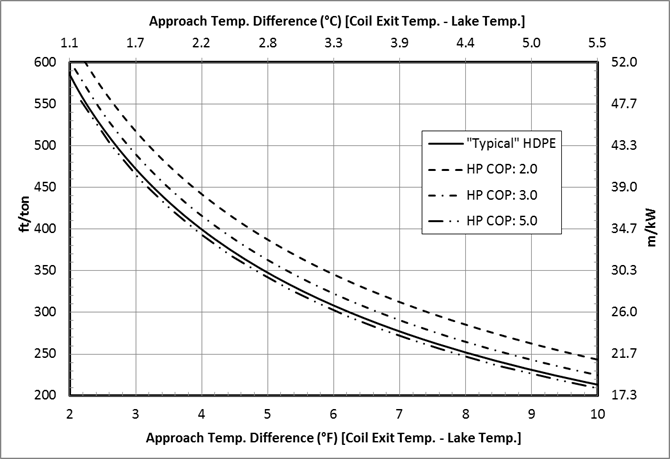
\includegraphics[width=0.8\textwidth]{HPCOP.png}
		\caption{Heat pump COP design diagram}
		\label{fig:DesignTools:SpcCooling:HPCOP}
	\end{figure}
	
Figure \ref{fig:DesignTools:SpcCooling:HPCOPPE} shows the percent error between the ``typical" case and the different fixed heat pump COP cases. From the ``typical" case which was a fixed heat pump COP of 4.0, selecting a heat pump with a COP of 2.0 will require a 7-13\% increase in installed pipe length to meet the same cooling load. For the heat pump with a fixed COP of 3.0, an increase in installed pipe of about 2-4\% should be implimented. Selecting a more efficient heat pump with a COP of 5.0, a decrease in required pipe length of 2-3\% can be realized. 
	
	\begin{figure}
		\centering
		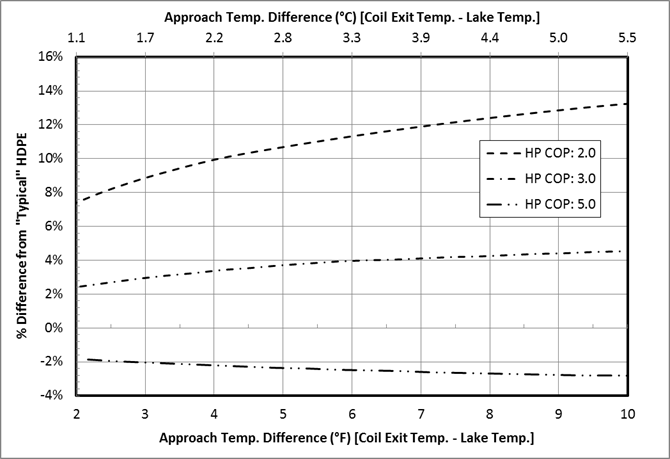
\includegraphics[width=0.8\textwidth]{HPCOPPE.png}
		\caption{Heat pump COP design diagram percent error}
		\label{fig:DesignTools:SpcCooling:HPCOPPE}
	\end{figure}


Figure \ref{fig:DesignTools:SpcCooling:PipeSize} shows how varying the pipe size on the ``typical" HDPE case affects coil sizing. All parameters are identical to the ``typical" HDPE case with the exception of the nominal pipe diameter as indicated in the figure. Figure \ref{fig:DesignTools:SpcCooling:PipeSizePE} shows the percent difference between the ``typical" case and the cases with 3/4 in.\ (19 mm) and 1-1/4 in.\ (32 mm) pipe sizes.

	\begin{figure}
		\centering
		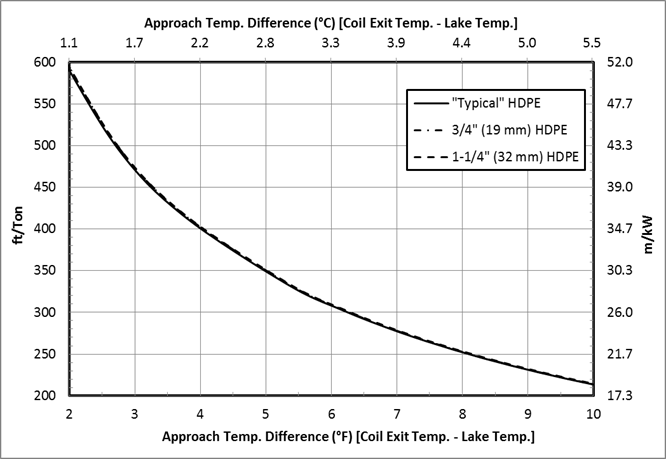
\includegraphics[width=0.8\textwidth]{PipeSize.png}
		\caption{Pipe size design diagram}
		\label{fig:DesignTools:SpcCooling:PipeSize}
	\end{figure}
	
From Figure \ref{fig:DesignTools:SpcCooling:PipeSize}, we can see that changing the nominal pipe diameter has a very small influence on heat exchanger sizing when compared to the base case. Nominal differences across the range of approach temperatures are minimal which can be seen in Figure \ref{fig:DesignTools:SpcCooling:PipeSizePE}. 
	
	\begin{figure}
		\centering
		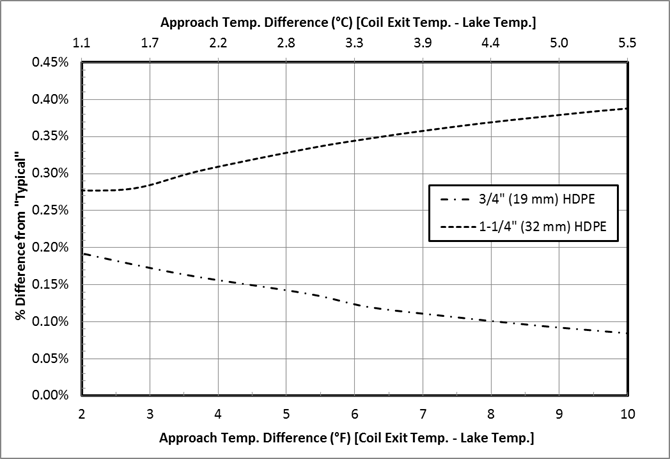
\includegraphics[width=0.8\textwidth]{PipeSizePE.png}
		\caption{Pipe size design diagram percent error}
		\label{fig:DesignTools:SpcCooling:PipeSizePE}
	\end{figure}
	
The reason that changing pipe size has little effect is due to the fact that any increase in pipe size, and thus surface area, $A_s$, is offset by a decrease in convection coefficients. We also know from previously as was shown with Equation \ref{eq:ExpResult:Uncertainty:DoDi} that the ratio $D_0/D_i$ will be constant, and therefore, so too will pipe conduction resistance. Table \ref{tab:DesignTools:SpcCooling:PipeSize:Params} below shows the convection coefficients, surface areas, and combined conductance values for the data used to generate Figure \ref{fig:DesignTools:SpcCooling:PipeSize} at an approach temperature of 6$^\circ$F (3.3$^\circ$C). Here, we see that exactly what was described. As surface area increases, the convection coefficient decreases. As a result, the combined conductances are nearly equal to each other.
	
	\begin{table}[h]
		\centering
		\caption{Convection coefficients and SWHE surface areas at 6$^\circ$F (3.3$^\circ$C) approach temperature for Figure \ref{fig:DesignTools:SpcCooling:PipeSize} }
		\label{tab:DesignTools:SpcCooling:PipeSize:Params}
		\begin{tabular}{c | c | c | c | c | c }
			\hline
			Pipe Size & $h_o$ & $h_i$ & $A,s,o$ & $A,s,i$ & $\left((h_o A,s,o)^{-1} + (h_i A,s,i)^{-1}\right)^{-1}$ \\
			\hline
			 & $W/m^2K$ & $W/m^2K$ & $m^2$ & $m^2$ & $W/K$ \\
			\hline	\hline	
			3/4 in.\ & \multirow{2}{*}{364} & \multirow{2}{*}{1677} & \multirow{2}{*}{8.0} & \multirow{2}{*}{6.4} & \multirow{2}{*}{2281} \\
			(19 mm) & & & & & \\
			\hline
			1 in.\ & \multirow{2}{*}{307} & \multirow{2}{*}{1131} & \multirow{2}{*}{10.0} & \multirow{2}{*}{8.0} & \multirow{2}{*}{2286} \\
			(25 mm) & & & & & \\
			\hline
			1-1/4 in.\ & \multirow{2}{*}{257} & \multirow{2}{*}{753} & \multirow{2}{*}{12.6} & \multirow{2}{*}{10.2} & \multirow{2}{*}{2280} \\
			(32 mm) & & & & & \\
			\hline
		\end{tabular}
	\end{table}
	
Figure \ref{fig:DesignTools:SpcCooling:VertHorizSpacing} shows the variation on the base case when the largest and smallest horizontal/vertical tube-to-tube spacing is applied. All other parameters are identical to the ``typical" HDPE case with the exception of the horizontal and vertical tube-tube spacing as indicated in the figure.

	\begin{figure}
		\centering
		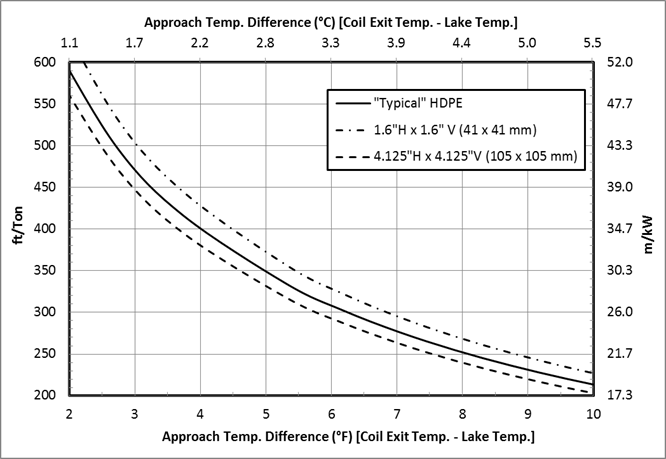
\includegraphics[width=0.8\textwidth]{VertHorizSpacing.png}
		\caption{Vertical and horizontal spacing design diagram}
		\label{fig:DesignTools:SpcCooling:VertHorizSpacing}
	\end{figure}
	
From Figure \ref{fig:DesignTools:SpcCooling:VertHorizSpacing}, we see that variations in horizontal/vertical tube-tube spacing has a larger impact on the base case. This is attributed entirely to the change in outside convective resistance. The nominal difference is constant across the range of approach temperature differences at $\pm$6\% which is visible in Figure \ref{fig:DesignTools:SpcCooling:VertHorizSpacingPE}.
	
	\begin{figure}
		\centering
		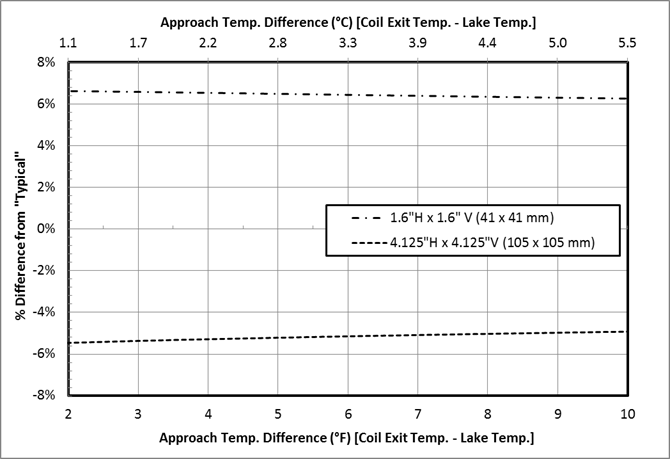
\includegraphics[width=0.8\textwidth]{VertHorizSpacingPE.png}
		\caption{Vertical and horizontal spacing design diagram percent error}
		\label{fig:DesignTools:SpcCooling:VertHorizSpacingPE}
	\end{figure}
	


Figure \ref{fig:DesignTools:SpcCooling:CircFluid} shows the variation in the base case when circulating fluid is varied. All other parameters are identical to the ``typical" case with the exception of the circulating fluid as indicated in the figure.

	\begin{figure}
		\centering
		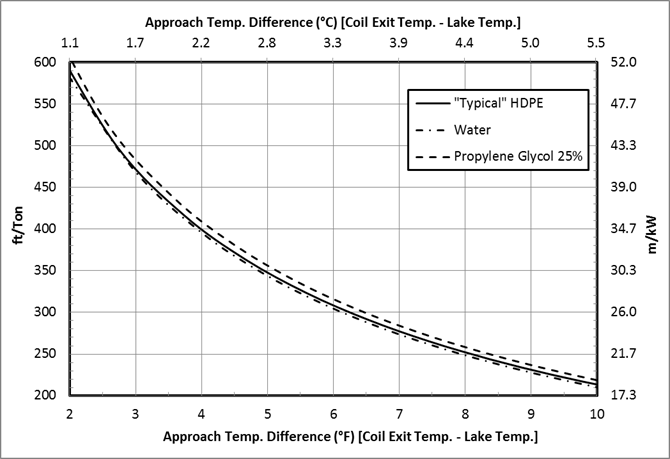
\includegraphics[width=0.8\textwidth]{CircFluid.png}
		\caption{Circulating fluid comparison design diagram}
		\label{fig:DesignTools:SpcCooling:CircFluid}
	\end{figure}
	
In Figure \ref{fig:DesignTools:SpcCooling:CircFluid}, we can see that circulating fluid has a relatively small effect on the base case. Water is more thermally conductive, less viscous, has a higher specific heat, and is less dense when compared to 25\% PG solution. For water, the combined effects result in a higher Reynolds number which is inversely proportional to inside convective resistance, and lower Prandtl number when compared to 25\% PG solution. Since Prandtl number can be described as the ratio of viscous diffusion to thermal diffusion, lower Prandtl numbers imply a better propensity for thermal diffusion. Hence, we expect that the pure water circulating fluid to perform better than any given concentration of PG solution. The nominal difference between the ``typical" case and the circulating fluid variations is $\pm$2\% which can be seen in Figure \ref{fig:DesignTools:SpcCooling:CircFluidPE}.	
	
	\begin{figure}
		\centering
		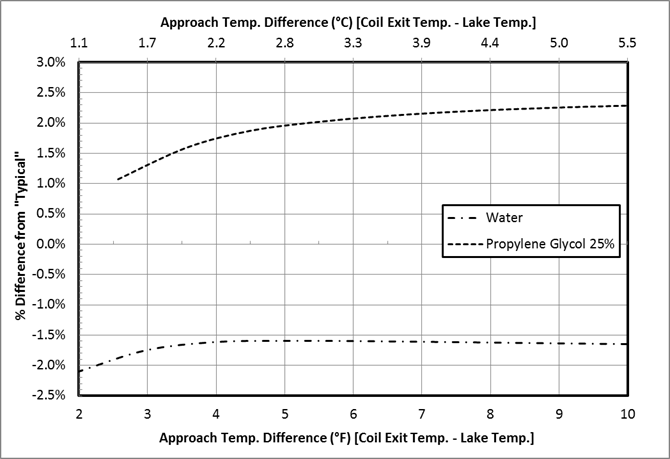
\includegraphics[width=0.8\textwidth]{CircFluidPE.png}
		\caption{Circulating fluid comparison design diagram percent error}
		\label{fig:DesignTools:SpcCooling:CircFluidPE}
	\end{figure}
	
Figure \ref{fig:DesignTools:SpcCooling:FlowRate} shows the variation in the base case when circulating fluid flow rate is varied. All other parameters are identical to the ``typical" case with the exception of the circulating fluid flow rate.

	\begin{figure}
		\centering
		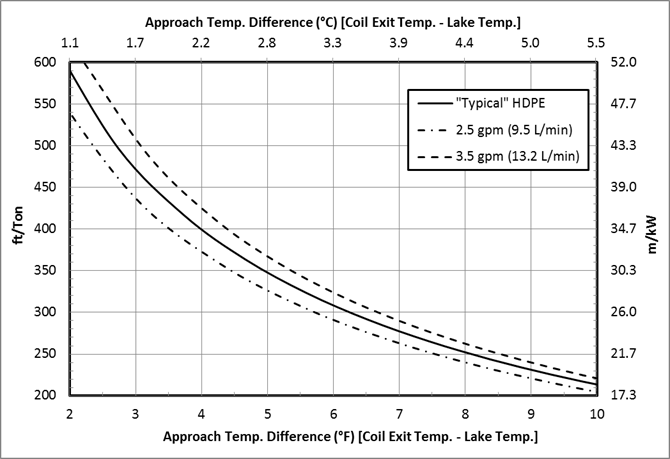
\includegraphics[width=0.8\textwidth]{FlowRate.png}
		\caption{Flow rate comparison design diagram}
		\label{fig:DesignTools:SpcCooling:FlowRate}
	\end{figure}
	
Because it may seem counter intuitive that increasing the flow rate will require a longer tube, a brief explanation is given. The SWHE is modeled as a heat exchanger with either the log-mean temperature difference (LMTD) method, or the effectiveness-NTU ($\varepsilon$-NTU) method. In our case, the LMTD method is used, however, all information is also available to verify the $\varepsilon$-NTU method. 
To understand why the required pipe length increases with increasing mass flow rate, we must understand that for all cases Equation \ref{eq:DesignTools:SpcCooling:HeatBal} must be satisfied.

	\begin{equation}
		\dot{Q}=\mbox{UA} \Delta T_{lm} = \dot{m} c_{p,f} (T_{in}-T_{out})
		\label{eq:DesignTools:SpcCooling:HeatBal}
	\end{equation}
	
In our case, heat transfer rate is fixed. For any given approach temperature difference, the outlet temperature between the cases is also fixed due to the approach temperature definition. If we look at the right side of the equation, increasing mass flow rate requires a decrease in inlet temperature for a fixed heat transfer rate and fixed exiting fluid temperature. If the inlet temperature drops, the $\Delta T$ across the HX will therefore decrease which causes LMTD to drop. Again, in order to satisfy the constant heat transfer condition, UA must then increase in order to balance the heat. 

UA will increase in two ways. The first is due to increasing the U value from the increase in mass flow rate. This causes internal convective resistance to decease. The second is the increase in surface area. Therefore, heat exchanger length must increase with increasing flow rate to maintain the same approach temperature difference. We can see this behavior from the following data outlined in Table \ref{tab:DesignTools:SpcCooling:FlowRateParams} which is taken from the calculations used to create Figure \ref{fig:DesignTools:SpcCooling:FlowRate} at an approach temperature of 8$^\circ$F (4.4$^\circ$C). The lake temperature is 70$^\circ$F (21.1$^\circ$C) with a heat pump COP of 4.0.

	\begin{table}[h]
		\centering
		\caption[Parameters used in Figure \ref{fig:DesignTools:SpcCooling:FlowRate}]{Parameters taken from the data used to generate Figure \ref{fig:DesignTools:SpcCooling:FlowRate} at an approach temperature of 8$^\circ$F (4.4$^\circ$C)}
		\label{tab:DesignTools:SpcCooling:FlowRateParams}
		\begin{tabular}{r | c c c}
		\hline
		\multirow{2}{*}{Parameter} & 2.5 gpm & 3.0 gpm & 3.5 gpm \\
		& (9.5 L/min) & (11.4 L/min) & (13.2 L/min) \\
		\hline\hline
		$\Delta T_{LM}$ [$^\circ$C] & 7.33 & 6.90 & 6.59 \\
		\hline
		$T_{out}$ [$^\circ$C] & \multicolumn{3}{c}{25.6} \\
		\hline
		$T_{in}$ [$^\circ$C] & 32.4 & 31.3 & 30.4 \\
		\hline
		$T_{out}-T_{in}$ [$^\circ$C] & 6.8 & 5.7 & 4.9\\
		\hline
		UA [W/K] & 599 & 638 & 668 \\
		\hline
		$A_{s,o}$ [m$^2$] & 7.68 & 8.08 & 8.39 \\
		\hline
		$A_{s,i}$ [m$^2$] & 6.20 & 6.52 & 6.78 \\
		\hline
		$h_o$ [W/m$^2$K] & 327 & 323 & 320 \\
		\hline
		$h_i$ [W/m$^2$K] & 990 & 1149 & 1305 \\
		\hline
		L [m] & 73.2 & 77.0 & 80.0 \\
		\hline
		$\dot{m}c_{p,f}$ [W/K] & 643 & 771 & 900 \\
		\hline
		$\varepsilon$ & 0.61 & 0.56 & 0.52 \\
		\hline
		NTU & 0.933 & 0.827 & 0.743 \\
		\hline
		$Q_{space}$ [W] & \multicolumn{3}{c}{3517} \\
		\hline
		$Q_{coil}$ [W] & \multicolumn{3}{c}{4396} \\
		\hline
		$Q_{max}$ [W] & 7251 & 7822 & 8394 \\
		\hline
		\end{tabular}
	\end{table}
	
From the table, we can verify that in order to maintain a given approach temperature, we must increase tube length. This behavior is essentially an artifact of the approach temperature definition and the way in which the design diagrams are derived. In a real system, increasing flow rate will decrease the temperature drop across the coil but it will also increase system capacity due to the increase in mass flow rate.

As and example to demonstrate the effect of increasing flow rate, if we take the ``typical" case at an approach temperature difference of 8$^\circ$F (4.4$^\circ$C), the approach temperature will need to increase to roughly 8.5$^\circ$F (4.7$^\circ$C) if the flow rate is increased to 3.5 gpm (13.2 L/min). This is determined by taking the ``typical" case at a 8$^\circ$F (4.4$^\circ$C) approach temperature and following horizontally until the 3.5 gpm (13.2 L/min) line is intersected at approximately 8.5$^\circ$F (4.7$^\circ$C) approach temperature.

Figure \ref{fig:DesignTools:SpcCooling:FlowRatePE} shows the percent difference from the different flow rate scenarios against the base case. At the lowest end of the approach temperature difference range, the percent difference ranges from +6\% to -8\%, while near the upper end of the approach temperature difference range, the percent differences range from +3\% to -4\%. Depending on the desired approach temperature difference, the designer should appropriately determine the percent correction required, depending on their situation.

	\begin{figure}
		\centering
		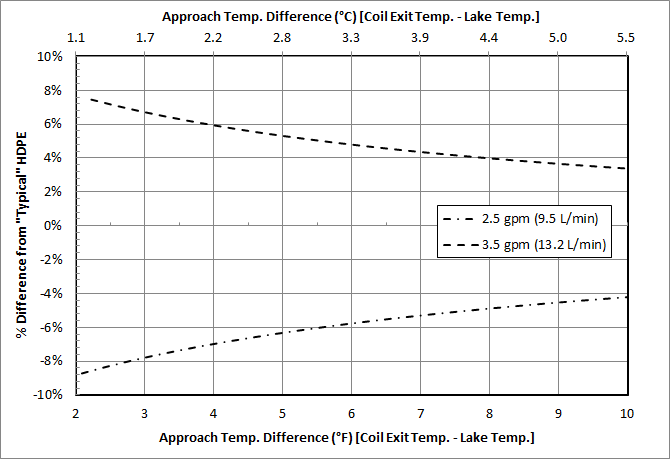
\includegraphics[width=0.8\textwidth]{FlowRatePE.png}
		\caption{Flow rate comparison design diagram percent error}
		\label{fig:DesignTools:SpcCooling:FlowRatePE}
	\end{figure}

Figure \ref{fig:DesignTools:SpcCooling:TubeMaterial} shows the variation in the base case when tube material is varied. All other parameters are identical to the ``typical" case with the exception of the tube material as indicated in the figure.

	\begin{figure}
		\centering
		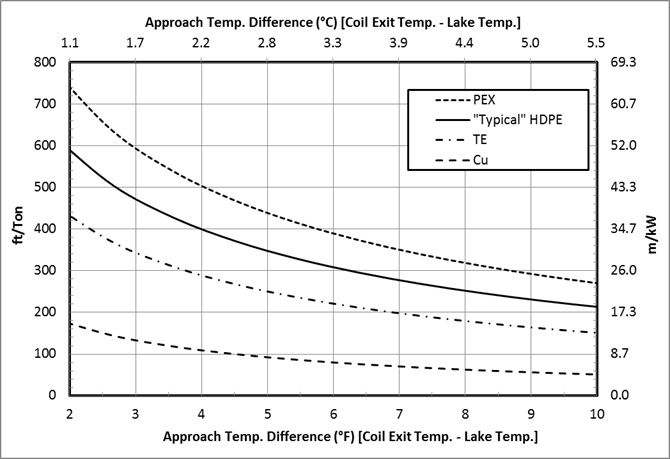
\includegraphics[width=0.8\textwidth]{TubeMaterial.png}
		\caption{Tube material comparison design diagram}
		\label{fig:DesignTools:SpcCooling:TubeMaterial}
	\end{figure}
	
We can see from Figure \ref{fig:DesignTools:SpcCooling:TubeMaterial} that tube material has a significant effect on required heat exchanger size. Cross linked polyethylene (PEX) is not recommended for obvious reasons. Thermal conductivity is similar to standard PE 3408 HDPE; however, the tube walls are much thicker which adds even more to the already dominant thermal resistance of the tube wall. Thermally enhanced HDPE is geometrically identical to the standard SDR-11 HDPE, however, it has a thermal conductivity that is 75\% higher than that of standard HDPE. This reduces its thermal resistance and makes it an attractive alternative to standard HDPE. Copper obviously has a thermal conductivity that is much higher than standard HDPE. This makes it attractive from a heat transfer perspective, but from a financial or durability perspective designers should exercise caution.

From the base case 25\% should be added if PEX piping is selected. A reduction of 30\% of coil length can be realized if the thermally enhanced HDPE is used. A 70\% reduction in required coil length can be expected if copper tubing is used. This can be seen for the given range of approach temperatures in Figure \ref{fig:DesignTools:SpcCooling:TubeMaterialPE}.

	\begin{figure}
		\centering
		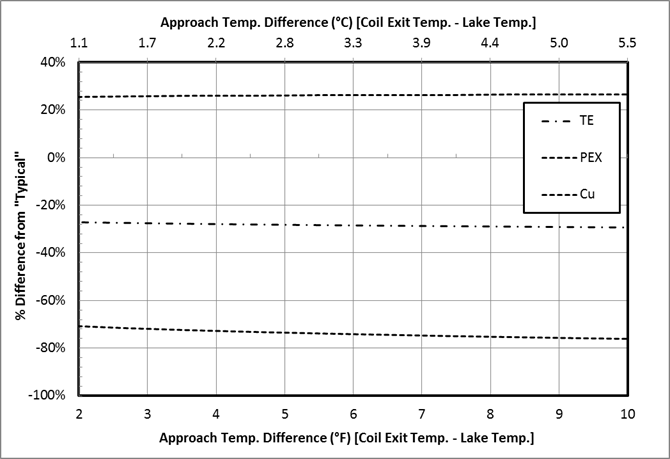
\includegraphics[width=0.8\textwidth]{TubeMaterialPE.png}
		\caption{Tube material comparison design diagram percent error}
		\label{fig:DesignTools:SpcCooling:TubeMaterialPE}
	\end{figure}

Figure \ref{fig:DesignTools:SpcCooling:TubeSchedule} shows the variation in the base case when tube schedule is varied. All other parameters are identical to the ``typical" case with the exception of the tube schedule as indicated in the figure.

	\begin{figure}
		\centering
		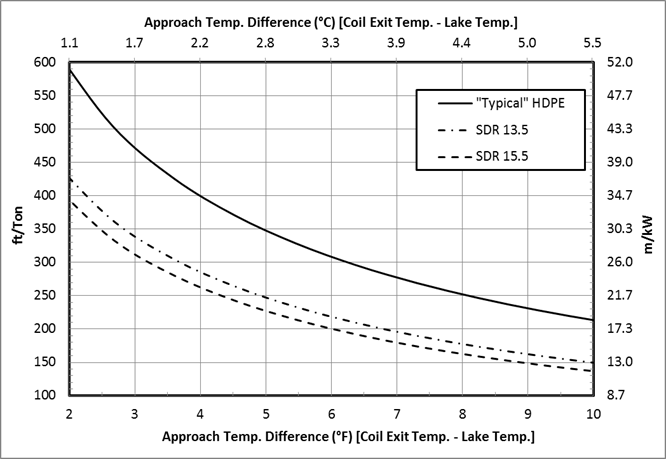
\includegraphics[width=0.8\textwidth]{TubeSchedule.png}
		\caption[Tube schedule comparison design diagram]{Design diagram indicating differences between different tubing schedules}
		\label{fig:DesignTools:SpcCooling:TubeSchedule}
	\end{figure}
	
From Figure \ref{fig:DesignTools:SpcCooling:TubeSchedule} we can see that tube schedule also plays a large role in required system size. From Chapter \ref{ch:ExpResult}, we see that the pipe can account for 60-70\% of the total thermal resistance. Any reduction in this will decrease required system length. Designers can expect reductions in required length of around 29\% and 35\% for SDR-13.5 and SDR-15.5 pipe schedules, respectively. This is visible in Figure \ref{fig:DesignTools:SpcCooling:TubeSchedulePE} over the range of given approach temperatures.

The thinner pipe, though, should be considered carefully from a durability stand point. SDR-11 HDPE is quite durable; however cases have been reported where SWHE failures have occurred due to tidal action which cause the pipes to rub on other tubes and structures. Thinner pipe walls will only lead to failure sooner if the SWHE is expected to be abraded by its surroundings.

	\begin{figure}
		\centering
		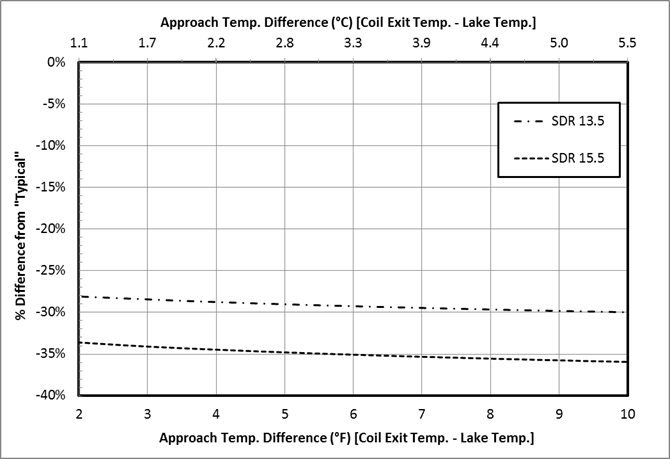
\includegraphics[width=0.8\textwidth]{TubeSchedulePE.png}
		\caption[Tube schedule comparison design diagram percent error]{Design diagram indicating differences between different tubing schedules}
		\label{fig:DesignTools:SpcCooling:TubeSchedulePE}
	\end{figure}

Figure \ref{fig:DesignTools:SpcCooling:HDPEFouling} shows the variation in the base case when tube external fouling is considered. All other parameters are identical to the ``typical" case with the exception of the fouling as indicated in the figure.

	\begin{figure}
		\centering
		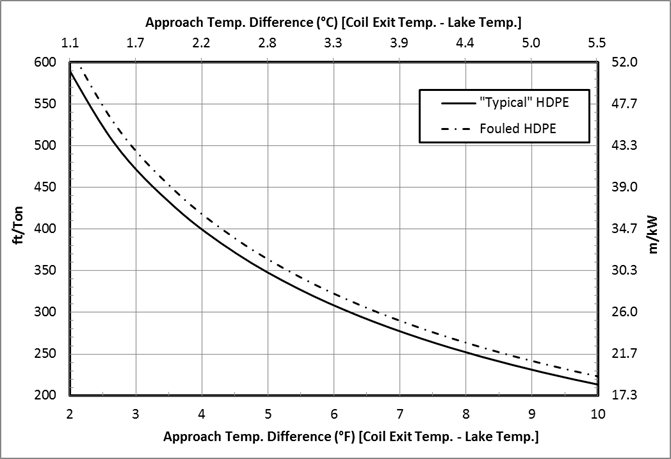
\includegraphics[width=0.8\textwidth]{HDPEFouling.png}
		\caption{HDPE external fouling comparison design diagram}
		\label{fig:DesignTools:SpcCooling:HDPEFouling}
	\end{figure}
	
Here we see that external fouling has a small effect on the HDPE tubing because it only constitutes a small portion of the overall thermal resistance. For the base HDPE case, an increase of 4\% would be required to overcome external fouling affects. This can be seen in Figure \ref{fig:DesignTools:SpcCooling:HDPEFoulingPE}. Fouling was taken as 0.003 hr-ft$^2$-$^\circ$F/BTU (0.00053 $m^2K/W$) for river water from \cite{Chenoweth1990}.

	\begin{figure}
		\centering
		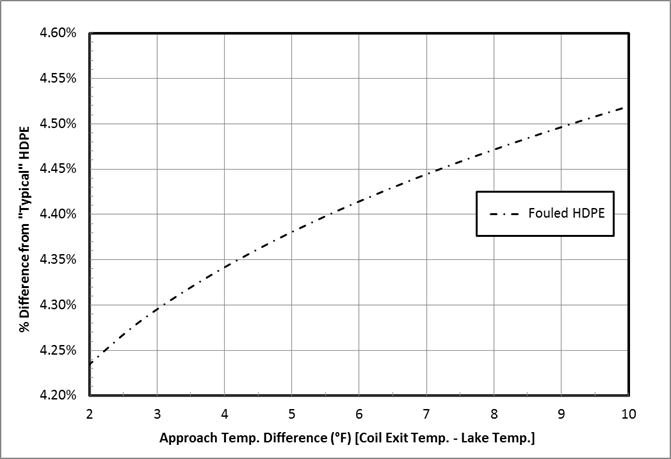
\includegraphics[width=0.8\textwidth]{HDPEFoulingPE.png}
		\caption{HDPE external fouling comparison design diagram percent error}
		\label{fig:DesignTools:SpcCooling:HDPEFoulingPE}
	\end{figure}

Figure \ref{fig:DesignTools:SpcCooling:CopperFouling} shows the variation in the copper type M case when the tube external surface is fouled. All other parameters are identical to the ``typical" case with the exception of the fouling and copper tubing material as indicated in the figure.

	\begin{figure}
		\centering
		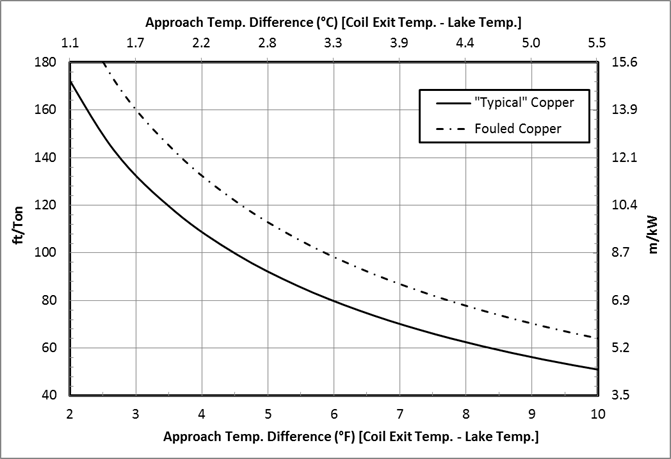
\includegraphics[width=0.8\textwidth]{CopperFouling.png}
		\caption{Copper external fouling comparison design diagram}
		\label{fig:DesignTools:SpcCooling:CopperFouling}
	\end{figure}
	
Here, fouling will have a much larger effect on copper piping because tube wall resistance is a much smaller portion of the total thermal resistance. For copper, we can expect a 19-26\% increase in required tube length from the lowest to highest approach temperatures indicated. The percent difference between the cases over the range of approach temperatures can be seen in Figure \ref{fig:DesignTools:SpcCooling:CopperFoulingPE}.

	\begin{figure}
		\centering
		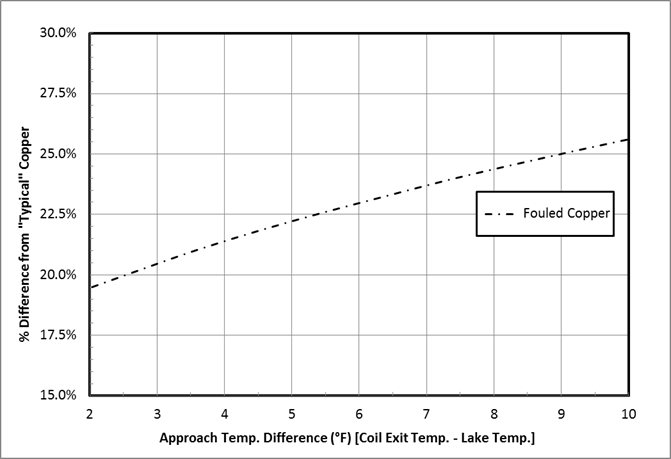
\includegraphics[width=0.8\textwidth]{CopperFoulingPE.png}
		\caption{Copper external fouling comparison design diagram percent error}
		\label{fig:DesignTools:SpcCooling:CopperFoulingPE}
	\end{figure}

Figure \ref{fig:DesignTools:SpcCooling:HDPEInsideFouling} shows the variation in the base case when the tube internal fouling is considered. All other parameters are identical to the ``typical" case with the exception of the internal fouling as indicated in the figure.

	\begin{figure}
		\centering
		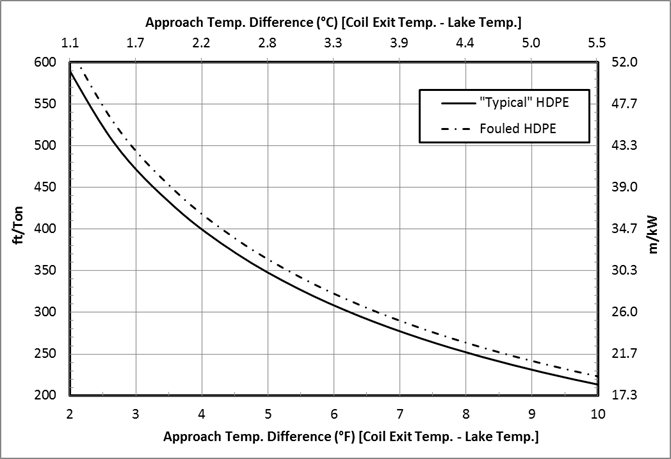
\includegraphics[width=0.8\textwidth]{HDPEFouling.png}
		\caption{HDPE internal fouling comparison design diagram}
		\label{fig:DesignTools:SpcCooling:HDPEInsideFouling}
	\end{figure}
	
As was the case with external fouling, we see that fouling has a small effect on the HDPE tubing because it only constitutes a small portion of the overall thermal resistance. From the base HDPE case, an increase of about 2\% would be required to overcome internal fouling affects. This can be seen in Figure \ref{fig:DesignTools:SpcCooling:HDPEInsideFoulingPE}. Fouling was taken as 0.001 hr-ft$^2$-$^\circ$F/BTU (0.000175 $m^2K/W$) for treated closed loop systems from \cite{Chenoweth1990}.

	\begin{figure}
		\centering
		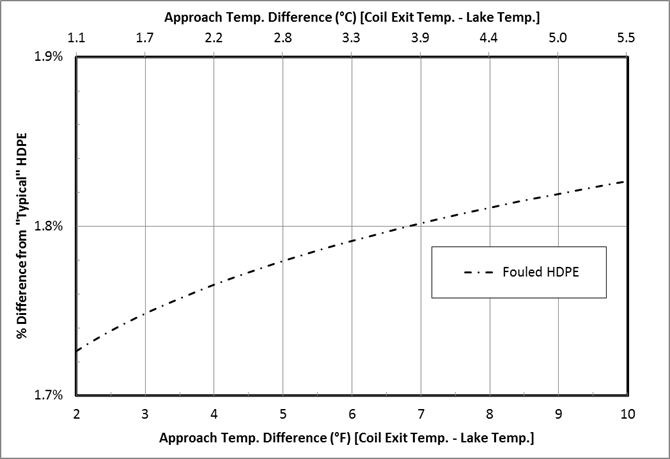
\includegraphics[width=0.8\textwidth]{HDPEInsideFoulingPE.png}
		\caption{HDPE internal fouling comparison design diagram percent error}
		\label{fig:DesignTools:SpcCooling:HDPEInsideFoulingPE}
	\end{figure}

Figure \ref{fig:DesignTools:SpcCooling:CopperInsideFouling} shows the variation in the copper type M case when the tube internal fouling is varied. All other parameters are identical to the ``typical" case with the exception of the internal fouling and copper tubing material as indicated in the figure.

	\begin{figure}
		\centering
		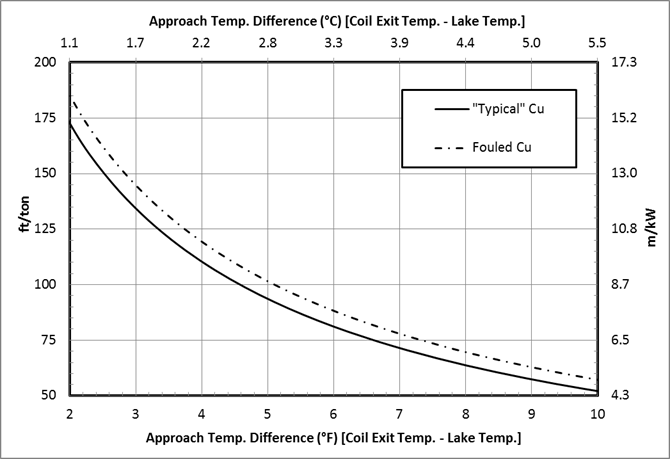
\includegraphics[width=0.8\textwidth]{CopperInsideFouling.png}
		\caption{Copper internal fouling comparison design diagram}
		\label{fig:DesignTools:SpcCooling:CopperInsideFouling}
	\end{figure}
	
Here again, fouling will have a much larger effect on copper piping because tube wall resistance is a much smaller portion of the total thermal resistance. For copper, we can expect about a 7-9\% increase in required tube length from the lowest to highest approach temperatures indicated. The percent difference between the cases over the range of approach temperatures can be seen in Figure \ref{fig:DesignTools:SpcCooling:CopperInsideFoulingPE}.

	\begin{figure}
		\centering
		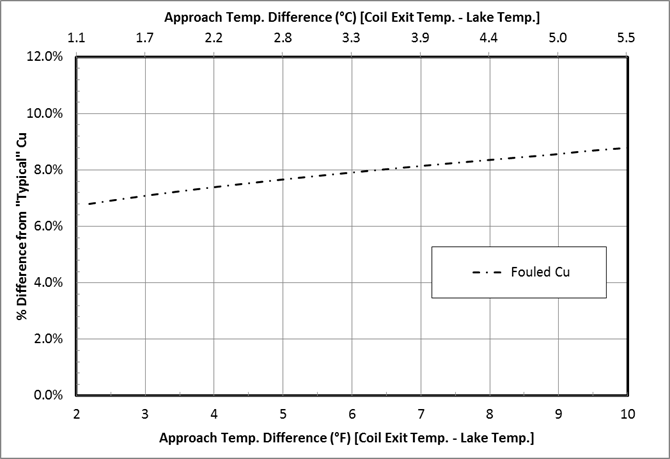
\includegraphics[width=0.8\textwidth]{CopperInsideFoulingPE.png}
		\caption{Copper internal fouling comparison design diagram percent error}
		\label{fig:DesignTools:SpcCooling:CopperInsideFoulingPE}
	\end{figure}

Figure \ref{fig:DesignTools:SpcCooling:LakeTemp} shows the variation in the ``typical" case when lake temperature is varied. All other parameters are identical to the ``typical" case with the exception of the lake temperature as indicated in the figure.

	\begin{figure}
		\centering
		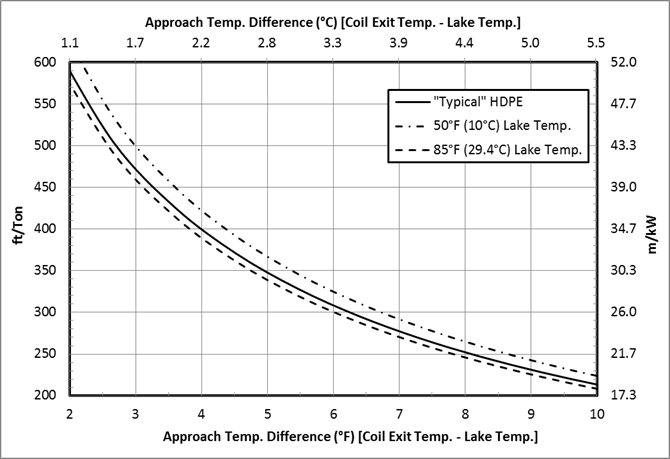
\includegraphics[width=0.8\textwidth]{LakeTemp.png}
		\caption{Lake temperature comparison design diagram}
		\label{fig:DesignTools:SpcCooling:LakeTemp}
	\end{figure}
	
The percent difference due to the effect of lake temperature variation can be seen in Figure \ref{fig:DesignTools:SpcCooling:LakeTempPE}.

	\begin{figure}
		\centering
		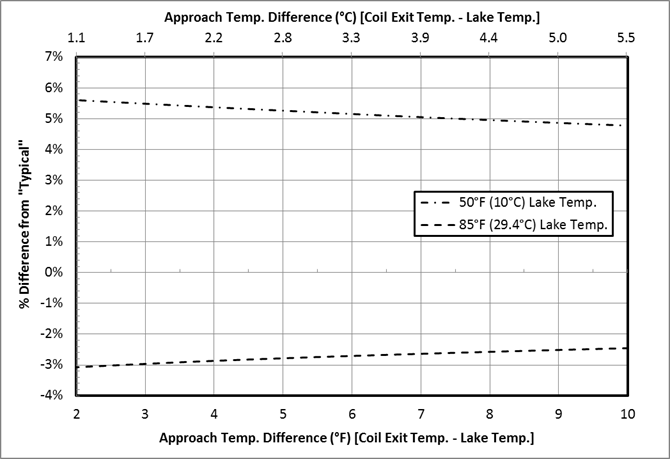
\includegraphics[width=0.8\textwidth]{LakeTempPE.png}
		\caption{Lake temperature comparison design diagram percent error}
		\label{fig:DesignTools:SpcCooling:LakeTempPE}
	\end{figure}
	
It may seem counter intuitive that an increase in lake temperature will cause a decrease in required coil length; however this is an artifact of the approach temperature difference definition and the method whereby the diagram was derived.

$\partial \rho / \partial T$, the derivative of the density of water with respect to temperature is greater at higher water temperatures than at lower water temperatures. This is an important fact to note because $\partial \rho / \partial T$ shows up in our calculations in the thermal coefficient of expansion, which is part of the Rayleigh number. Therefore, at higher lake temperatures, Rayleigh numbers will be higher and will predict a lower outside convection resistance when compared to lower lake temperatures, even though the approach temperature differences may be identical.

From a heat transfer perspective, we understand that lower lake temperatures are more favorable from a system point of view. Figure \ref{fig:DesignTools:SpcCooling:HPEFTIsotherm} shows the required coil length plotted against lake temperature for four separate heat pump entering fluid temperature (EFT) isotherms. All other parameters are identical to the ``typical" HDPE case. Here we can clearly see that lower lake temperatures are more favorable from a heat transfer perspective. For example, if we have 200 ft/ton (17.3 m/kW) of installed coil, for a lake temperature of 94$^\circ$F (34.4$^\circ$C), the heat pump EFT will be around 105$^\circ$F (40.6$^\circ$C) which is going to have a much lower heat pump COP when compared to a 64$^\circ$F (17.8$^\circ$C) lake which will have a 75$^\circ$F (23.9$^\circ$C) heat pump EFT. For the example, even though the approach temperatures are identical, overall system performance will be much better at lower lake temperatures.

	\begin{figure}
		\centering
		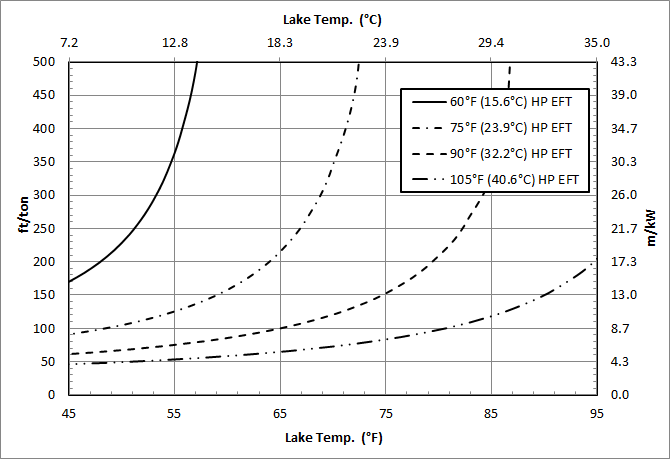
\includegraphics[width=0.8\textwidth]{HPEFTIsotherm.png}
		\caption[Heat pump EFT isotherm plot]{Heat pump EFT isotherm plot of required coil length plotted against lake temperature}
		\label{fig:DesignTools:SpcCooling:HPEFTIsotherm}
	\end{figure}
	
Designers could use this discussion to compare their application and lake temperature to the ``typical" lake temperature of 70$^\circ$F (21.1$^\circ$C) and then make a decision regarding how best to implement the results. If for example, the proposed design in in northern Canada and the lake temperature is not expected to exceed 50$^\circ$F (10$^\circ$C) during the cooling season, the designer may wish to consider increasing installed length by 5\% to account for the lower values of $\partial\rho/\partial T$ which occur at these temperatures. A designer in southern Florida, may consider the reverse.

Figure \ref{fig:DesignTools:SpcCooling:Quiescent} shows the variation in the ``typical" HDPE case when the lake is expected to have quiescent conditions, or by some other means convective motion is constrained. All other parameters are identical to the ``typical" HDPE case with the exception of the outside convection coefficient as was indicated in Section \ref{sec:Correlation:Conclusions}.
	
	\begin{figure}
		\centering
		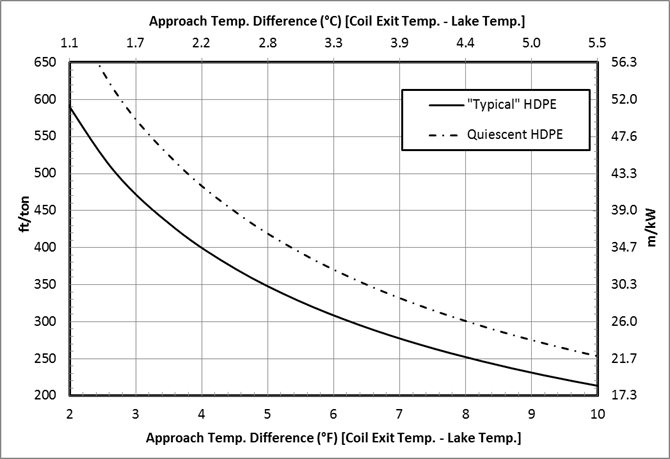
\includegraphics[width=0.8\textwidth]{Quiescent.png}
		\caption{Quiescent HDPE pond design diagram}
		\label{fig:DesignTools:SpcCooling:Quiescent}
	\end{figure}
	
The results indicated in this figure are a result of the differences in outside convective resistance base on the experimentally derived convection correlation from Chapter \ref{ch:Correlation}. Due to the increase in outside convective resistance, an increase in required installation length would be required if the system was expected to operate in a surface water body that constrained the convective motion. The percent difference from the ``typical" HDPE case across the range of approach temperatures can be seen in Figure \ref{fig:DesignTools:SpcCooling:QuiescentPE}.
	
	\begin{figure}
		\centering
		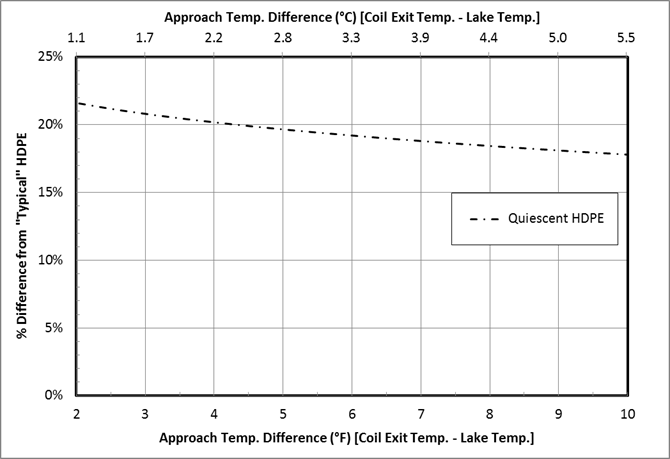
\includegraphics[width=0.8\textwidth]{QuiescentPE.png}
		\caption{Quiescent HDPE pond design diagram percent error}
		\label{fig:DesignTools:SpcCooling:QuiescentPE}
	\end{figure}
	
Figure \ref{fig:DesignTools:SpcCooling:QuiescentCopper} shows the variation in the ``typical" copper case when lake is expected to have quiescent conditions. All other parameters are identical to the ``typical" copper case with the exception of the outside convection coefficient as was indicated in Section \ref{sec:Correlation:Conclusions}.
	
	\begin{figure}
		\centering
		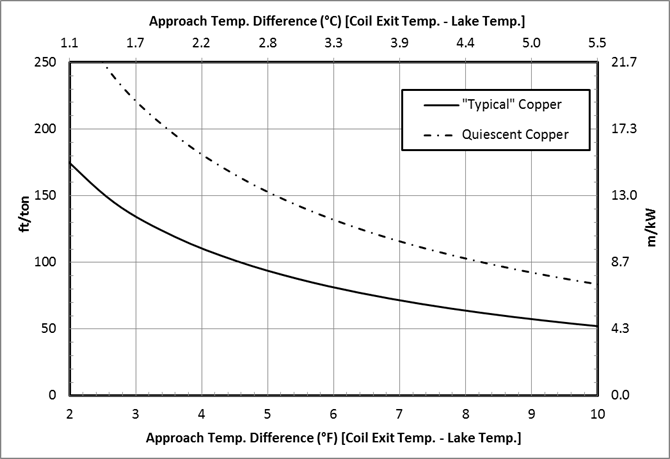
\includegraphics[width=0.8\textwidth]{QuiescentCopper.png}
		\caption{Quiescent copper pond design diagram}
		\label{fig:DesignTools:SpcCooling:QuiescentCopper}
	\end{figure}
	
Here, because the outside convective resistance is a much larger portion of the SHWEs total thermal resistance, an increase of installed pipe length of around 61\% would be required if quiescent conditions are expected to occur. Figure \ref{fig:DesignTools:SpcCooling:CopperFoulingPE} shows the percent difference from the ``typical" copper case over the range of given approach temperatures.
	
	\begin{figure}
		\centering
		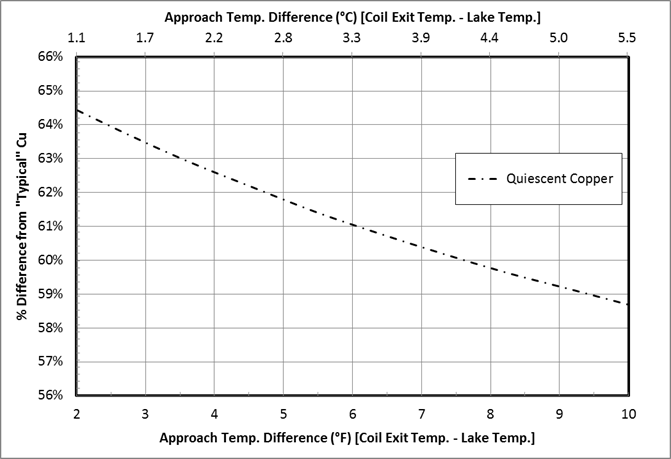
\includegraphics[width=0.8\textwidth]{QuiescentCopperPE.png}
		\caption{Quiescent copper pond design diagram percent error}
		\label{fig:DesignTools:SpcCooling:QuiescentCopperPE}
	\end{figure}


Tables \ref{tab:DesignTools:SpcCooling:PercentDiffSummaryHDPE} shows a summary of the percent change from the ``typical" HDPE case when comparing different design parameter variations for the same approach temperature difference. The table can be implemented by comparing a proposed design to the ``typicial" design. This can then be used to determine overall percent correction by using Equation \ref{eq:DesignTools:SpcCooling:PercentEqn}. This equation combines the percent error differences, $p$, from the different parameters into a single percent error correction factor, $P$.

	\begin{equation}
		P = (1+p_1)\cdot(1+p_2)\cdots(1+p_n)
		\label{eq:DesignTools:SpcCooling:PercentEqn}
	\end{equation}
	
As an example, the ``typical" case will be compared to the ``best" case. When compared to the ``typical" case, the ``best" case has a lower COP, higher lake temperature, larger tube size and larger tube-tube spacing, and water the circulating fluid. From Table \ref{tab:DesignTools:SpcCooling:PercentDiffSummaryHDPE}, we can see that an average percent difference for each respective parameter listed is, +3\% for lower COP, -3\% for higher lake temperature, -5\% for larger tube-tube spacing, and -2\% for water. These parameters are shown calculated in Equation \ref{eq:DesignTools:SpcCooling:PercentEqnExamp}. 

	\begin{equation}
		P_{best} = (1+0.03)\cdot(1-0.03)\cdot(1-0.05)\cdot(1-0.02) \approx 0.93
		\label{eq:DesignTools:SpcCooling:PercentEqnExamp}
	\end{equation}
	
The calculation results in an approximate decrease in required tube length of 7\% when comparing the ``best" case to the ``typical" case. This can be verified by the results shown in Figure \ref{fig:DesignTools:SpcCooling:BestWorstPE}, where the ``best" case is shown to be roughly 4-8\% below the ``typical" case.

%\pagebreak

	\begin{table}[h]
		\centering
		\caption[Percent change summary across all HDPE space cooling design diagrams]{Percent change from ``typical" HDPE case for different SWHE and SWHP system parameter variations based on space cooling conditions}
		\label{tab:DesignTools:SpcCooling:PercentDiffSummaryHDPE}
		\begin{tabular}{r c c}
		\hline
		Parameter & \% Diff. from ``typical" case & Notes\\
		\hline\hline
		HP $\mbox{COP}_h$: 2.0 & +7-13\% & \multirow{3}{*}{See Figure \ref{fig:DesignTools:SpcCooling:HPCOPPE}} \\
		HP $\mbox{COP}_h$: 3.0 & +2-4\% & \\
		HP $\mbox{COP}_h$: 5.0 & -2-3\% & \\
		\hline
		3/4 in.\ HDPE & $<$1\% & \\
		1-1/4 in.\ HDPE & $<$1\% & \\
		\hline
		Small Tube Spacing & +6\% & \\
		Large Tube Spacing & -5\% & \\
		\hline
		Water & -2\% & \\
		25\% PG & +2\% & \\
		\hline
		2.5 gpm & -8-4\% & \multirow{2}{*}{See Figure \ref{fig:DesignTools:SpcCooling:FlowRatePE}} \\
		3.5 gpm & +6-3\% & \\
		\hline
		PEX & +25\% & \\
		TEHDPE & -25\% & \\
		Copper & -70\% & \\
		\hline
		SDR 13.5 & -30\% & \\
		SDR 15.5 & -35\% & \\
		\hline
		External Fouling & +4\% & \\
		Internal Fouling & +2\% & \\
		\hline
		Low Lake Temp & +4\% & \\
		High Lake Temp & -3\% & \\
		\hline
		Quiescent Surface Water & +18-22\% & See Figure \ref{fig:DesignTools:SpcCooling:QuiescentPE}\\
		\hline		
		\end{tabular}
	\end{table}
	
Table \ref{tab:DesignTools:SpcCooling:PercentDiffSummaryCu} shows the percent change from the ``typical" copper case due to parameter variations. This table will give an estimate of the percent change from the ``typical" copper case due to external and internal fouling, as well as quiescent pond conditions.
	
	\begin{table}[h]
		\centering
		\caption[Percent change summary across all copper space cooling design diagrams]{Percent change from ``typical" copper case for different SWHE and SWHP system parameter variations based on space cooling}
		\label{tab:DesignTools:SpcCooling:PercentDiffSummaryCu}
		\begin{tabular}{r c c}
		\hline
		Parameter & \% Diff. from ``typical" case & Notes \\
		\hline\hline
		External Fouling & +19-26\% & See Figure \ref{fig:DesignTools:SpcCooling:CopperFoulingPE} \\
		Internal Fouling & +7-9\% & See Figure \ref{fig:DesignTools:SpcCooling:CopperInsideFoulingPE} \\
		\hline
		Quiescent Surface Water & +59-64\% & See Figure \ref{fig:DesignTools:SpcCooling:QuiescentCopperPE}\\
		\hline
		
		\end{tabular}
	\end{table}

\section{Space Heating Design Graphs}
\label{sec:DesignTools:SpcHeating}

Space heating presents some significant challenges when it comes to designing surface water heat pump systems. This is due to the fact heat must be extracted from the surface water in order to provide space heating. The first law of thermodynamics tells us that in order to extract heat from the surface water body, the SWHE circulating fluid temperature must be lower than the surface water temperature. Lowering the circulating fluid temperature can become problematic if the temperature is dropped below the freezing point of water. As was shown in Chapter \ref{ch:ExpResult}, dropping the circulating fluid temperature below the freezing point of the surface water body can cause ice-on-coil freezing. Should enough ice build on the SWHE, system performance will decrease. Potential SWHE damage could also occur if the SWHE becomes buoyant and begins to float.

When compared to systems used for space heating, space cooling systems are not inherently safe from a system design perspective. If a SWHE for a space cooling system is undersized, circulating fluid temperatures will rise until the heat transfer rate between the system and the lake are balanced. However, for space heating applications, an undersized system will cause loop temperatures to drop, possibly below the freezing point of the surface water. This potentially could cause icing which can reduce system performance or damage the SWHE.

In this section, no ``typical" design case will be given. Only the most conservative estimates of what can be done in the region prior to coil icing. Also, no information will be given for sizing coils under ice-on-coil freezing conditions.

Figure \ref{fig:DesignTools:SpcHeating:LakeTempSpcHeating} shows a lake temperature isotherm plot showing required coil length plotted against approach temperature difference. Table \ref{tab:DesignTools:SpcHeating:LakeTempSpcHeatingParams} shows the SHWE and SWHP system parameters used to generate Figure \ref{fig:DesignTools:SpcHeating:LakeTempSpcHeating}.

	\begin{figure}
		\centering
		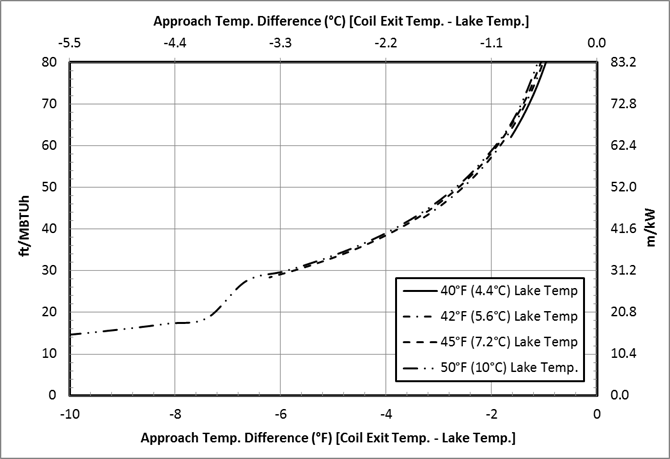
\includegraphics[width=0.8\textwidth]{LakeTempSpcHeating.png}
		\caption{Space heating design diagram for HDPE SWHE}
		\label{fig:DesignTools:SpcHeating:LakeTempSpcHeating}
	\end{figure}
	
For the 50$^\circ$F (10$^\circ$C) lake temperature curve, the sharp decrease in required pipe length below an approach temperature of -7$^\circ$ (-4$^\circ$C) is due to the discontinuous nature of the convection correlation for heat extraction. This behavior was described in Section \ref{subsec:Correlation:PoolHeatExtr}.

	\begin{table}[h]
		\centering
		\caption{SWHE and SWHP system parameters used to generate Figure \ref{fig:DesignTools:SpcHeating:LakeTempSpcHeating}}
		\label{tab:DesignTools:SpcHeating:LakeTempSpcHeatingParams}
		\begin{tabular}{r c c c c}
		\hline
		\multirow{2}{*}{Lake Temp} & 40$^\circ$F & 42$^\circ$F & 45$^\circ$F & 50$^\circ$F \\
		& (4.4$^\circ$C) & (5.6$^\circ$C) & (7.2$^\circ$C) & (10$^\circ$C) \\
		\hline\hline
		HP $\mbox{COP}_c$ & 2.9 & 3.2 & 3.5 & 3.8 \\
		\hline
		\multirow{2}{*}{Tube Spacing} & \multicolumn{4}{c}{4.125 in.\ H x 4.125 in.\ V} \\
		& \multicolumn{4}{c}{(105 mm x 105 mm)} \\
		\hline
		Tube Size & \multicolumn{4}{c}{3/4 in.\ (19 mm)} \\
		\hline
		Tube Material & \multicolumn{4}{c}{HDPE} \\
		\hline
		Flow Rate & \multicolumn{4}{c}{3 gpm (11.4 L/min)} \\
		\hline
		Space Heating & \multicolumn{4}{c}{12,000 BTU/h (3,517 W)} \\
		\hline
		Circulating Fluid & \multicolumn{4}{c}{12.5\% Propylene Glycol} \\
		\hline
		Fouling & \multicolumn{4}{c}{None} \\
		\hline
		SW Correlation & \multicolumn{4}{c}{Pond} \\
		\hline
		\end{tabular}
	\end{table}
	
A similar diagram was created for copper heat exchangers. This is shown below in Figure \ref{fig:DesignTools:SpcHeating:LakeTempSpcHeatingCopper}. All parameters are identical to the parameters shown in Table \ref{tab:DesignTools:SpcHeating:LakeTempSpcHeatingParams} with the exception of the tube material, which was changed to copper, and tube size which was changed to a 1 in.\ (25 mm) nominal Type M tube size.
	
	\begin{figure}
		\centering
		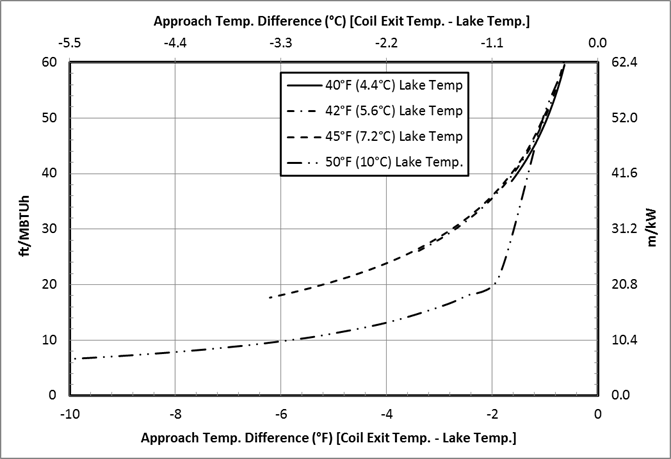
\includegraphics[width=0.8\textwidth]{LakeTempSpcHeatingCopper.png}
		\caption{Space heating design diagram for copper SWHE}
		\label{fig:DesignTools:SpcHeating:LakeTempSpcHeatingCopper}
	\end{figure}
	
Here again, the 50$^\circ$F (10$^\circ$C) lake temperature curve indicates the discontinuous nature of the convection correlation for heat extraction. As was the case with the HDPE design diagram, the outside Rayleigh numbers for the lake temperature curves less than 50$^\circ$F (10$^\circ$C)  never exceed $Ra_D^* = 1 \cdot 10^6$. Comparing the HDPE and copper diagrams shows, as expected, that the copper coil length could be reduced if copper is selected. 
	
Extrapolation beyond the lower limit of the curves provided in Figures \ref{fig:DesignTools:SpcHeating:LakeTempSpcHeating} and \ref{fig:DesignTools:SpcHeating:LakeTempSpcHeatingCopper} is not permitted due to the fact that coil freezing may occur which would cause system performance to decrease. Also, if sufficient ice is allowed to form on the coil, the buoyant forces may tear the coil free from its anchors, potentially damaging or destroying the surface water heat exchanger.

From our experience, coiled heat exchangers perform with relatively little performance degradation under initial icing conditions, so long as the ice forming on the tube surface has not intersected the ice forming on adjacent tube surfaces. However, if the gap between the tubes is allowed to bridge, the heat exchanger essentially becomes a solid block of ice eliminating surface water flow between the tubes. Outside convective resistance will become so large that no heat transfer will be able to take place.

One method that may allow for continued operation when lake temperatures drop to unfavorably low levels is to increase the circulating fluid flow rate. This could be used for lakes where the lake temperature is only expected to drop to dangerously low temperatures for a small period of time. Increasing the circulating fluid flow rate will allow operation at extended temperatures up to a certain point. Figure \ref{fig:DesignTools:SpcHeating:ApprTempSpcHeating} shows an approach temperature difference isotherm plot of minimum lake temperature as a function of circulating fluid flow rate. For Figure 9-14, coil inlet temperatures were set at 32.5$^\circ$F so as to avoid coil icing.

	\begin{figure}
		\centering
		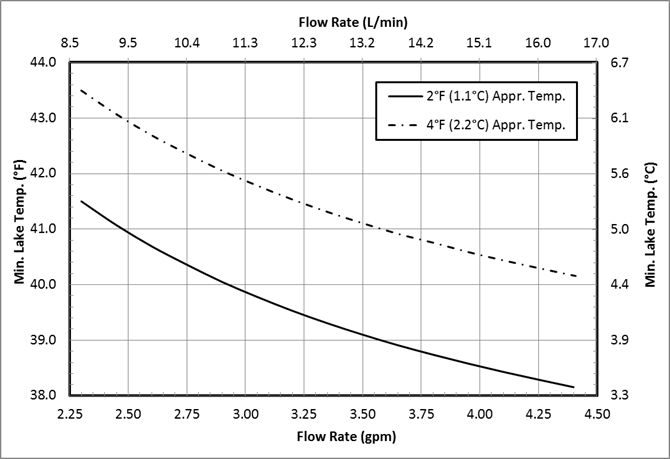
\includegraphics[width=0.8\textwidth]{ApprTempSpcHeating.png}
		\caption[Approach temperature isotherm for space heating]{Approach temperature isotherm plot of minimum lake temperature plotted against required flow rate}
		\label{fig:DesignTools:SpcHeating:ApprTempSpcHeating}
	\end{figure}

We can see from Figure \ref{fig:DesignTools:SpcHeating:ApprTempSpcHeating} that increasing fluid flow rate may allow for operation at lower lake temperatures, but only to a certain extent. The additional energy expended pumping the fluid at a higher flow rate may be equal to, or greater than the energy required to add the necessary supplementary heating.

The companion to Figure \ref{fig:DesignTools:SpcHeating:ApprTempSpcHeating} which was taken from the same simulation is Figure \ref{fig:DesignTools:SpcHeating:ApprTemp2SpcHeating}. This figure shows the tube length required at the given lake and approach temperatures to meet the zone heating load.

	\begin{figure}
		\centering
		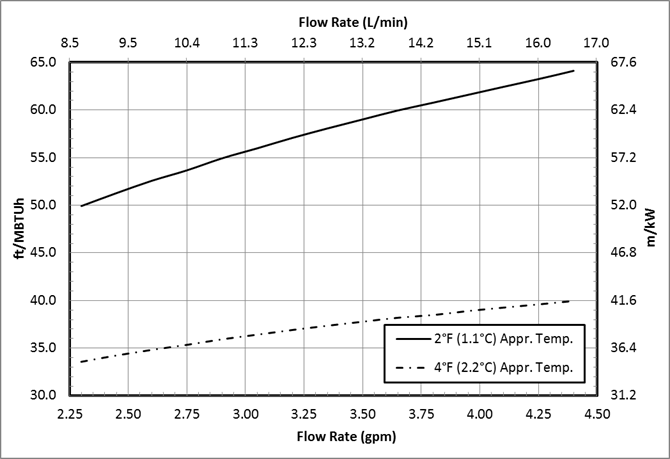
\includegraphics[width=0.8\textwidth]{ApprTemp2SpcHeating.png}
		\caption[Approach temperature isotherm for space heating]{Approach temperature isotherm plot of required tube length plotted against required flow rate}
		\label{fig:DesignTools:SpcHeating:ApprTemp2SpcHeating}
	\end{figure}

As a general recommendation, coil tube-tube spacing should be kept at as great a distance as possible if the potential for icing exists. This will allow for the greatest safety factor if high heating periods are encountered and some freezing occurs. However, if the designer determines that under their given circumstances, coil icing is likely, supplementary heating should be provided or other heat exchanger designs should be explored.

